\documentclass{article} % For LaTeX2e
\usepackage{../../tex-style/nips_2014,times}
\usepackage{hyperref}
\usepackage{url}
\usepackage{graphicx}
\usepackage{CJKutf8}
\hypersetup{unicode}
\AtBeginShipoutFirst{\input{zhwinfonts.tex}}

\title{机器学习及其在图像处理中的应用}

\author{
 \url{http://www.dosrc.com/}
}


\newcommand{\fix}{\marginpar{FIX}}
\newcommand{\new}{\marginpar{NEW}}


\nipsfinalcopy % Uncomment for camera-ready version

\begin{document}
\begin{CJK*}{UTF8}{gkai}

\maketitle

\begin{abstract}
本文为读书报告,介绍了机器学期的两个大的分支概率图模型和深度学习,其中概率图模型主要介绍了什么是概率图模型,怎么表示,独立性相关概念。文中介绍了概率图模型中两个主要的模型,有向图的贝叶斯模型和无向图的马尔可夫模型以及马尔可夫模型在图像处理中的应用。深度学习方面介绍了两个重要的模型BP神经网络和卷神经网络,稍微介绍了递归神经网络。卷积神经网络在图像识别上应用的非常广泛,文末介绍了如何将卷积神经网络应用与图像目标检测,并阐述了卷积神经网络的现实意义。
\end{abstract}

\section{概率图模型简介}
表示、推理和学习是构建智能系统的关键部分,概率图模型是能支持这三种功能的极少框架之一。

概率图模型分为用有向图表示的贝叶斯网络和用无向图表示的马尔可夫网,这两种模型表示都给出了独立关系和因子分解的对偶型。

\subsection*{如何表示}
我们的目的是在某个随机变量的集合 $\chi =\lbrace X _{1},\cdots X _{n} \rbrace$ 上表示联合分布概率P。原来的联合分布需要列出每个变量的变化组合,在表达方式上不够紧凑,考虑到随机变量的集合中存在一些独立变量或者条件独立变量,可以将这些变量分隔开来,这个想法类似于分隔噪声域的思想,因为相对独立变量之间的取值互相不产生影响。贝叶斯网络的表达方式如下图1所示

\begin{figure}[h]
\begin{center}

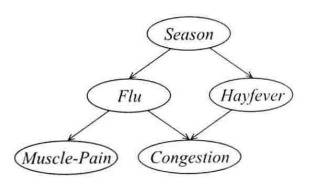
\includegraphics[width=2in]{1.png}

\end{center}
\caption{概率图模型的贝叶斯网图}
\end{figure}

当独立变量的个数增多时,联合分布表的表达方式规模会呈指数级增大。而采用概率图模型的因子分解方式表示将独立变量或条件独立变量分隔开来,将规模计算中的乘法转换为加法,表达方式紧凑。此外将相对独立的变量分隔开带来了另外一个好处就是表达更加模块化,这样当需要增加一个新的变量时,只要这个变量不是对所有其它的变量都产生影响就可以局部的更新概率图模型,但是联合分布表则必须整体的更新,这一性质使得概率图模型更加贴近真实世界,对模拟真实系统非常有价值。

\section{贝叶斯网络模型}
\subsection{朴素贝叶斯模型}
朴素贝叶斯模型假设所有的事例属于若干类中的一个,这些类包含所有情况且两两互斥,如下图2所示

\begin{figure}[h]
\begin{center}

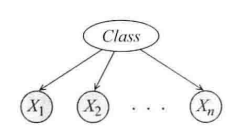
\includegraphics[width=1.5in]{2.png}
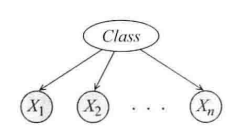
\includegraphics[width=1.5in]{2.png}

\end{center}
\caption{朴素贝叶斯模型的贝叶斯网图}
\end{figure}

该模型主要用于分类,此时注意朴素贝叶斯模型的前提假设是只能属于其中的一个类别,我们可以计算出分类决策的可信度,即模型相对于类$C^{2}$偏好于另一个类别$C^{1}$的程度。

\begin{equation}
\frac{P \left( C=c^{1}\vert x_{1},\cdots,x_{n} \right)}{P \left( C=c^{2}\vert x_{1},\cdots,x_{n} \right)} = \frac{P \left( C=c^{1} \right)}{P \left( C=c^{2} \right)}\prod_{i=1}^n \frac{P \left( x_{i}\vert C=c^{1} \right)}{P \left( x_{i}\vert C=c^{2} \right)}
\end{equation}

\subsection{贝叶斯模型}
贝叶斯网与朴素贝叶斯模型一样都是通过利用分布的独立性来获得紧凑且自然的表示,相对于朴素贝叶斯模型,贝叶斯网不必满足那些强独立性假设,贝叶斯网允许我们根据当前设置中出现的独立性质灵活的表示概率分布。

\subsubsection{模型表示}
贝叶斯网的表示核心是一个有向无圈图(DGA),其节点为论域中的随机变量,并且在直观上,其边表示一个节点对另外一个节点的直接影响。

\begin{figure}[h]
\begin{center}

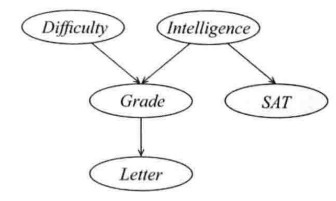
\includegraphics[width=2in]{3.png}

\end{center}
\caption{贝叶斯模型网图}
\end{figure}

上图3中表示学生的成绩(Grade)取决于课程的难度(Difficult)和学生的智商(Intelligence),推荐信的好坏只取决于学生的成绩(Grade),学生的SAT成绩只取决于学生的智商(Intelligence)。在该模型图中,除根节点外每个变量都关联着一个条件概率分布(根节点也可以看做条件为空的条件概率)。那么这一模型的联合概率分布就可以表示为各个节点的给定父节点的条件概率的乘积:
\begin{equation}
P\left( D,I,G,S,L \right )=P\left( D \right )P\left( I \right )P\left( G \vert D,I \right )P\left( S \vert I \right )P\left( L \vert G \right )
\end{equation}

更一般的写法为:
\begin{equation}
P\left( X _{1},\cdots,X _{n} \right )=\prod_{i=1}^n P\left( X _{i} \vert Pa ^{G}_{X _{i}} \right )
\end{equation}
这个等式也叫做贝叶斯链式法则,单个因子$P\left( X _{i} \vert Pa ^{G}_{X _{i}} \right )$称为条件概率分布(CPD)或局部概率模型。

\subsubsection{模型推理}
模型推理是从结果推理原因,在上图3的例子中就是比如知道了考试成绩(Grade)推理学生的智商(Intelligence),这一过程又叫做解释,表示为$P\left( I \vert G \right)$。

如果此学生的成绩较低我们可能会认为他的智商也比较低的概率会比较高,但是如果知道了课程的难度很高的话,那么就会让我们将他的智商比较低的概率减小,这一现象就做解释消除,解释消除是因果推理的一般模式的一个示例。

\subsubsection{贝叶斯网络的独立性}
在图3中,给定父节点G时,L与网中的所有其他节点条件独立:
\begin{equation}
\left( L \bot I,D,S \vert G \right)
\end{equation}
也就是说,一旦知道了学生的成绩,关于他的推荐信的好坏的可信度就不会被其他任何变量提供的信息所影响。图3中类似的独立性还有给定父节点I时,S与网络中其他节点条件独立:
\begin{equation}
\left( S \bot D,G,L \vert I \right)
\end{equation}
但是并不是只要给定父节点,节点就会与其他所有的节点条件独立,如图3中,给定I,D节点,G与L并不是条件独立的,事实上有:给定父节点,节点与所有它的非后代节点条件独立,表示为如下:

对每个变量$X _{i}:\left( X _{i} \bot NonDescendants \vert Pa ^{G} _{X _{i}} \right)$

NonDescendants表示$X _{i}$的非后代节点,$Pa ^{G} _{X _{i}}$表示$X _{i}$的父节点

注意,图3中,给定G的情况下,D和I并不是条件独立的,事实上D和I是独立的,但不是关于G条件独立的,这是因为G并不是D或I的父节点,这里千万不能弄混了。

\section{马尔可夫网络模型}
马尔可夫模型用于我们不能对变量之间的交互影响自然指定方向的各种现象,这些模型对于建模非常有用,而且,根据模型的独立性结构和推理任务,无向图模型还为我们提供了与有向图模型不同但通常更为简单的观点。

考虑如下的例子
\begin{figure}[h]
\begin{center}

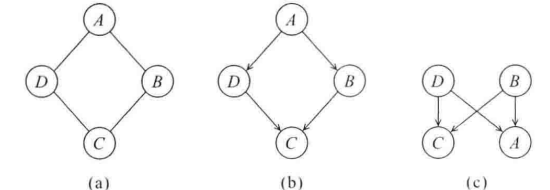
\includegraphics[width=3in]{4.png}

\end{center}
\caption{贝叶斯模型无法表示的独立性}
\end{figure}

在图4(a)中我们无法用贝叶斯模型同时表示$\left( B,D \bot A,C \right)$,$\left( A,C \bot B,D \right)$这两种独立性关系,图4(b),图4(c)是做的一些尝试,显然都无法满足要求,注意此处要求是有向无环图。这就需要用到马尔可夫网来表示。
\subsection{模型表示}
\begin{figure}[h]
\begin{center}

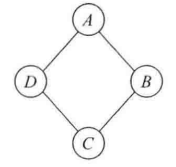
\includegraphics[width=1.5in]{5.png}

\end{center}
\caption{马尔可夫模型网图}
\end{figure}

同贝叶斯网一样,马尔可夫网中的节点代表变量,而边则与近邻变量之间的有向概率交互影响的概念相对应,这是一种不受网络中任何其他变量影响的交互影响。由于图中的交互影响是无向的,所以我们需要更加对称的参数化方法,直观上我们想要表示的是相关变量之间的亲密关系。比如,我们可能希望表示A和B之间意见一致性比意见分歧的可能性更大这一事实。我们把A、B与一个具有通用目标的函数联系起来,这个函数也称为一个因子。
假设因D表示随机变量的集合,因子$\phi$定义为从Val(D)映射到实数域R的一个函数。假如因子的所有表值均非负,那么这个因子称为非负的。变量集D称为因子的辖域,记为$Scope[\phi]$。
那么如何定义概率分布呢,我们非常期望将$P \left( a,b,c,d \right)$分解为$\phi _{1} \left( a,b \right) \cdot \phi _{2} \left( b,c \right) \cdot \phi _{3} \left( c,d \right) \cdot \phi _{4} \left( d,a \right)$,不过在这种情形下,并不能保证由这个过程获得的结果是一个归一化的联合概率分布。因此,我们首先通过将局部因子相乘来定义这个分布,然后将其归一化,从而使其成为一个合法的分布,定义如下:
\begin{equation}
P \left( a,b,c,d \right)=\frac{1}{Z} \phi _{1} \left( a,b \right) \cdot \phi _{2} \left( b,c \right) \cdot \phi _{3} \left( c,d \right) \cdot \phi _{4} \left( d,a \right)
\end{equation}
其中
\[Z=\sum _{a,b,c,d} \phi _{1} \left( a,b \right) \cdot \phi _{2} \left( b,c \right) \cdot \phi _{3} \left( c,d \right) \cdot \phi _{4} \left( d,a \right)\]
是一个归一化的常数,通常称为配分函数。
这种表示的好处是它对于我们表示变量之间的交互影响给予了极大的灵活性。如果希望改变A与B之间的交互影响的类型,那么无需处理归一化约束以及其他因子的交互影响,只要修改那个因子中的表值即可,但是直观上理解这些改变的作用往往很难。

\subsection{参数化}
为了表示分布,就像用CPD参数化有向图那样,我们需要给图结构关联一个参数集。但是因子既不能理解成概率,也不能看成条件概率,所以马尔可夫网的参数化不像贝叶斯网的参数化那样直观明了。参数化马尔可夫网的一个核心问题是,这种表示是无向的,因此参数化在本质上也不应该是有向的。

我们使用上面提到的因子来参数化马儿可夫网,但是若把因子定义为成对的顶点之间(也就是边)的函数则根本没有足够的数值可以将整个联合分布的空间覆盖,而且这样的因子只能描述成对变量的交互影响,而不能描述包含比较大的变量子集的值的组合的交互影响。所以我们把因子定义为在任何变量子集上来获得,并且定义一些因子的主要运算如下:
\begin{equation}
\psi \left( X,Y,Z \right) = \phi _{1} \left( X,Y \right) \cdot \phi _{2} \left( Y,Z \right)
\end{equation}

CPD和联合概率分布都是因子,实际上,贝叶斯网的链式法则将联合分布的因子定义为CPD因子的乘积。因此如果令$\phi _{X _{i}} \left( X _{i},Pa _{X _{i}} \right)$表示$P \left( X _{i} \vert Pa _{X _{i}} \right)$那么
\begin{equation}
P \left( X _{1}, \cdots ,X _{n} \right)=\prod _{i} \phi _{X _{i}}
\end{equation}

\subsection*{吉布斯分布}
现在可以更一般的用因子的乘积来定义分布的无向参数化,定义分布$P_{\phi}$ 
\begin{equation}
P_{\phi} \left( X _{1}, \cdots ,X _{n} \right)=\frac{1}{Z} \tilde{P}_{\phi} \left( X_{1},\cdots,X{n} \right)
\end{equation}
其中
\begin{equation}
\tilde{P}_{\phi} \left( X_{1},\cdots,X{n} \right)=\phi_{1}\left(D_{1}\right)\times\phi_{2}\left(D_{2}\right)\times\cdots\times\phi_{m}\left(D_{m}\right)
\end{equation}
是非归一化的度量,并且
\begin{equation}
Z=\sum_{X_{i},\cdots,X_{n}}\tilde{P}_{\phi} \left( X_{1},\cdots,X{n} \right)
\end{equation}
是配分函数的归一化常数,那么分布$\tilde{P}_{\phi}$称为由因子集$\phi=\left\lbrace \phi_{1}\left(D_{1}\right),\cdots,\phi_{K}\left(D_{K}\right)\right\rbrace$参数化的吉布斯分布
\subsection{马尔可夫网在图像处理中的应用}

马尔可夫网在计算机视觉中属于一个重要的应用领域,通常在计算机视觉中称为马尔可夫随机场,被广泛应用于多种视觉处理的任务中,如图像分割,去模糊和去噪,三维重建,物体识别等。在大部分应用中,网络以成对的MRF的形式呈现,变量对应于像素,而边也就是因子对应于表示图像上相邻像素之间的交互影响。这样除边界外每个像素都有四个相邻的节点。根据所处理任务的不同变量的取值空间,因子的形式也会不一样。这些模型通常用能量(对因子或节点的值的函数取负的对数)来表示,这些值代表了惩罚。

例如在图像分割中,我们的目的是将图像中的像素分割成与场景的不同部分分别对应的区域,在多类别的分隔中,每个变量$X_{i}$有一个域$\left\lbrace 1,\cdots,K\right\rbrace$,其中$X_{i}$的值表示像素i的一个区域分配(如天空、草地、水、汽车)。由于分类每个像素的的计算代价太大,我们可以用现有的方法先将图像分隔成一些超级像素也就是连贯的小区域,然后再对这些区域进行分类,每个小区域中所有的像素的类别都是一样的。通过超级像素我们可以导出一个图,在该途中,若超级像素之间相邻,我们就在他们之间画一条边。这样我们就可以定义出一个马尔可夫图分布了。

接着我们为每个超级像素提取特征,在图像分割中,特征通常包括颜色、纹理和地点等统计信息,为了降低维度,通常会对这些超级像素进行聚类。用于模型的特征就是这些聚类的结果的值,超级像素的节点位势(节点值的函数)就是这些特征的一个函数。定义这个模型的因子取决于图像中像素的具体的值,所以每个图像在这些超级像素的分隔标签上定义了一个不同的概率分布,这里用到的模型就是条件随机场。

模型在每队相邻的超级像素$X_{i}$和$X_{j}$之间包含了一对边位势。我们可以对这个位势用惩罚$\lambda $来刻画邻接的偏好。比如我们通常认为老虎更有可能在水的附近而不是蔬菜附近,为了刻画水在蔬菜的下方、汽车在路的上面以及天空位于所有的东西之上等常见的事实,我们可以让模型依赖于相关的像素位置,对于没有关系的超级像素,我们可以简单地对$X_{i}\neq X_{j}$定义一个惩罚值。

下图6是一个只包含单个像素上位势的模型(每个像素独立分类)导致的分隔结果和一个包含成对位势的模型产生的分隔结果的对比,这清楚的说明了对超级想的之间的相关性建模非常重要。
\begin{figure}[h]
\begin{center}

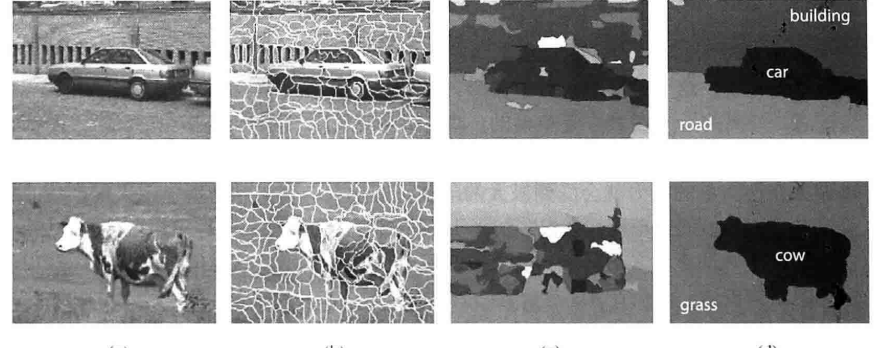
\includegraphics[width=6in]{6.png}

\end{center}
\caption{图像分割结果的连个例子}
\end{figure}

\section{深度学习}
深度学习是有别于概率图模型的机器学习研究的一个新的领域,它仿生人类的大脑神经网络的活动,构造具有多隐含层的神经网络结构,他不像概率图模型那样具有很强的可解释性,但是由于隐含层的存在它可以逼近任意复杂的函数,这就使得它的应用范围极其广泛。和概率图模型一样,深度学习使用的模型也是图模型。

\subsection{BP神经网络}
BP(Back Propagation)网络是由Rinehart和McClelland为首的科学家小组于1986年提出的,是一种按误差逆向传播算法训练的多层前馈网络,是目前应用最广泛的神经网络模型之一。BP网络能学习和存储大量的输入输出模式映射关系,而无需事前揭示描述这种映射关系的数学方程。它的学习规则是使用梯度下降法通过反向传播来不断调整网络的权值和阈值,使网络的误差平方和最小。BP神经网络模型拓扑结构如下图7:

\begin{figure}[h]
\begin{center}

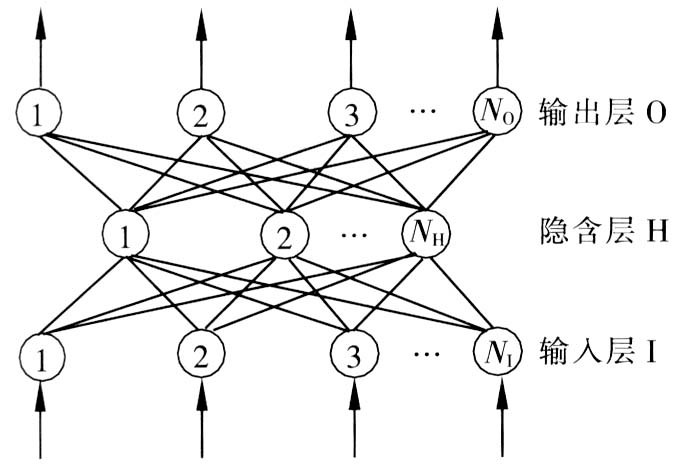
\includegraphics[width=2.5in]{7.jpg}

\end{center}
\caption{BP神经网络模型图}
\end{figure}
BP神经网络模型的拓扑结构包括输入层,隐藏层和输出层,其中输入层接收输入的参数将值传递给隐藏层,隐藏层通过对输入层的参数加权求和,并通过一个激活函数产生值传递给输出层,输出层通过对隐藏层传递来的值加权求和,同样也通过一个激活函数产生最终的输出。公式如下:

隐藏层的输出$z_{k}\left( k=1,2,\cdots N_{H} \right)$:
\begin{equation}
z_{k}=f_{1}\left( \sum_{i=1}^{N_{1}}v_{ki}x_{i} \right)
\end{equation}

输出层的输出$y_{j}\left( j=1,2,\cdots N_{0} \right)$:
\begin{equation} 
y_{j}=f_{2}\left( \sum_{k=1}^{N_{H}}w_{jk}z_{k} \right)
\end{equation}

BP神经网络产生输出后,通过和应有正确的输出对比,构造一个损失函数,就可以应用梯度下降法得到最佳的权重和,使得损失函数的值最小。这个过程称为误差的反向传播。

\subsection{卷积神经网络}
卷积神经网络中有两个重要的操作,一个是卷积操作,一个是池化。

\textbf{卷积:} 首先介绍下什么是卷积操作,卷积操作在对图像的处理中有所体现,对图像和滤波矩阵做内积的操作就是所谓的卷积操作,也是卷积神经网络的名字来源。通俗点讲就是图像每个点看做一个值,对一个矩形区域内的每个点乘以不同的权重值再求和得到一个新的值这就是卷积操作,矩形区域可以在图像上不断的移动就可以依次得到一系列新的点值,集合起来就是一幅新的图像,而权重值也可以表示为一个矩阵叫做卷积核,卷积神经网络为了节约参数数量,同样也秉承这图像上一部分的统计特性和其它部分是一样的,在整个图像的卷积操作中会保持卷积核不变,这也就是所谓的参数共享。虽然卷积核在卷积操作中保持不变,但是我们可以有多个卷积核,这样就能得到许多幅不同的图像,这些卷积而来的图像也叫作原图像的特征,不同的卷积核也就对应不同的特征提取方法。下图8为不同卷积核提取的特征(图片来源于网络):

\begin{figure}[h]
\begin{center}

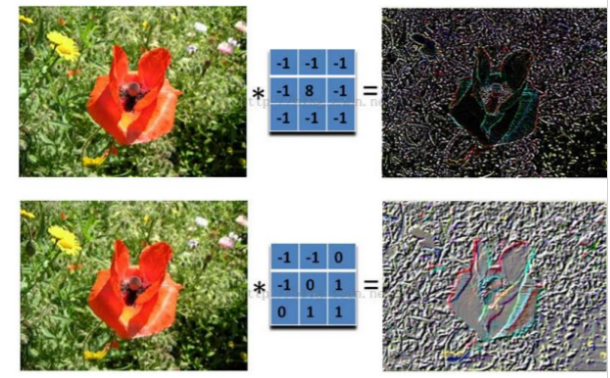
\includegraphics[width=4in]{8.png}

\end{center}
\caption{不同卷积核提取的特征}
\end{figure}

\textbf{池化:} 那么什么是池化呢,在通过卷积获取了图像的特征后,下一步我们希望利用这些特征去做分类,如果我们直接用提取到的特征去做分类的话,由于特征的维数过于巨大,这对于学习分类器的过程十分不便,并且容易出现过拟合的现象。为了解决这个问题,一个很自然的想法就是对不同位置的特征进行聚合统计。例如,我们可以计算图像一个区域上的某个特定特征的平均值或最大值,这些概要统计特征不仅具有低得多的维度,同时能改善结果。这种聚合的操作就叫做池化,根据计算池化的方法的不同,有时也叫作平均池化或者最大池化。下图9为最大池化(图片来源于网络):

\begin{figure}[h]
\begin{center}

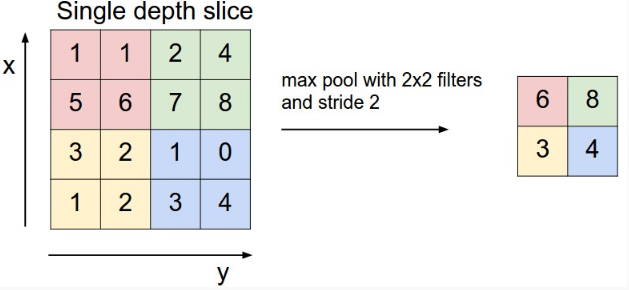
\includegraphics[width=4in]{9.png}

\end{center}
\caption{最大池化}
\end{figure}

\textbf{激活函数:}上面BP神经网络中的激活函数一般是sigmoid,但在实际梯度下降中,sigmoid激活函数容易导致饱和和终止梯度传递,也就是常说的梯度爆炸和梯度消失,在卷积神经网络中我们较常使用的是另外一个激活函数:ReLU,其图形表示如下图10:

\begin{figure}[h]
\begin{center}

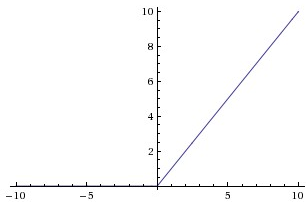
\includegraphics[width=2in]{10.png}

\end{center}
\caption{ReLU激活函数}
\end{figure}

这个激活函数形象的表示了折纸的过程,即将低维空间中线性不可分的一些点,通过对折到高维空间变成了线性可分。
\subsection{递归神经网络}
卷积神经网络隐藏层之间并没有联系,在递归神经网络中,隐藏层中的神经元可以有一条线连向自己,并附带一定的延迟,如一个或两个步长,这样当前的神经元就会接收来自两个地方的输入,一个是正常的输入,一个是上一个时间段神经元的输出,这样可以很好的表示历史信息,递归神经网络一般多用于自然语言处理中的翻译中,翻译不仅需要考虑当前的局部输入,还需要考虑当前句子之前的历史输入,总的来说递归神经网络是将某个时间序列转换为另外一个序列的过程。

\subsection{卷积神经网络在图像物体识别上的应用}
单一目标检测:单一目标检测问题可以转化为图像分类问题,就是从设定好的一组分类标签中选定一个标签分配给输入的图像。这就是计算机视觉的核心问题之一,尽管看似很简单,但是还是有许多各种各样的实际应用程序。例如单一目标检测,单一目标检测可以的使用神经网络通过提取图像的特征然后加以大量数据的训练学习就可以获得较高的目标检测准确率。

多目标检测:多目标检测不同于单目标检测,由于多目标图像中物体出现的数量不确定,位置不确定所以难度比单目标检测高很多。早期的多目标检测采用AdaBoost的方法,利用滑窗机制和多尺度可以比较好的解决多目标检测问题,卷积神经网络由于天然的带有滑动窗口机制和多尺度,因此可以非常方便的去处理多目标检测问题。
一个典型的目标检测架构如下图11(图像来源于PPT):

\begin{figure}[h]
\begin{center}

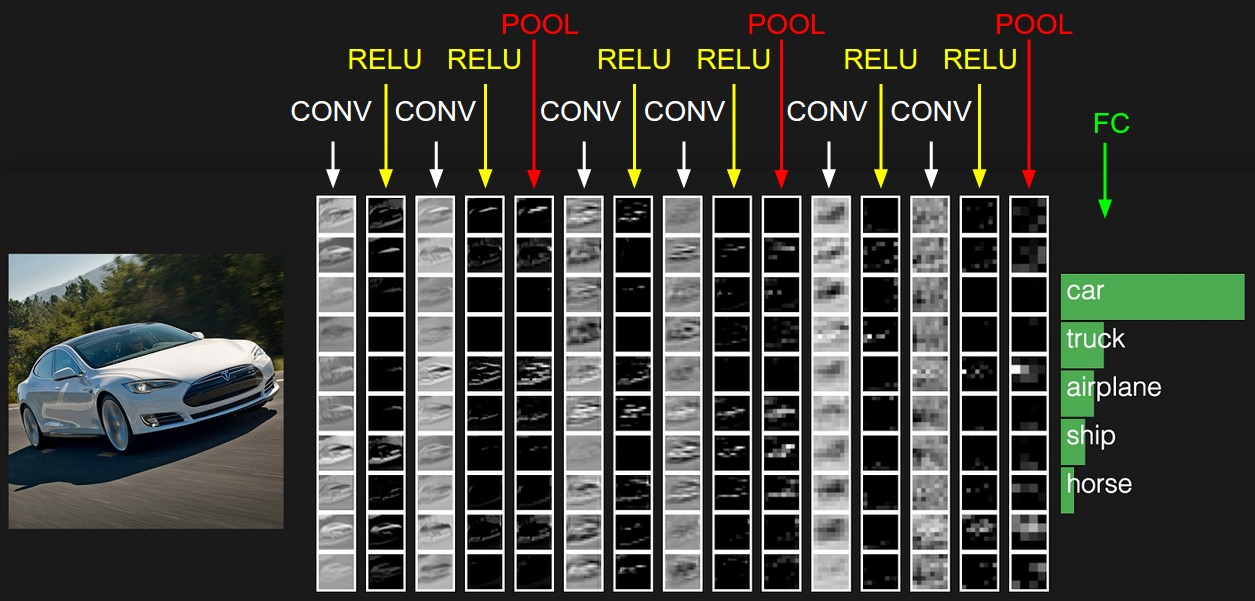
\includegraphics[width=5.5in]{11.png}

\end{center}
\caption{图像分类CNN架构}
\end{figure}

在该架构中,输入图像首先经过卷积操作,再输入到ReLU激活函数中也就是做折叠,再卷积再折叠,然后再经过一次池化,这样的步骤重复三次最后加个全连接层就能比较准确的识别出该图片为汽车。每次池化的过程中都可以接入一个全连接,由此可以产生出不同尺度的输出。

卷积操作看起来很是神秘,其实不然,只要想到这是一个特征提取的工具,例如检测人脸的时候,大概会构造这样一个卷积操作,就是用眉毛的像素减去眼睛的像素,或者用两只眼睛的像素减去鼻子的像素从而可以构造出人脸专有的特征,这就是卷积操作的现实意义,前面说了ReLU激活函数的作用为了更好将低维的一些分布映射到高维空间中去从而更加方便的进行分类,将非线性的关系转化为线性的关系。池化可以将相似的特征融合,从而可以降低数据的规模,让小数据可以反映大片数据。现在比较流行的是可变形的卷积操作,也就是卷积操作在学习过程中可以自我学习,不再需要是一个正方矩形,可以自己学习变为任意形状。


\subsubsection*{References}

\small{
[1](美)科勒(Koller, D), (以)弗里德曼(Friedman, N)著, 王飞跃, 韩素青译. 概率图模型 原理与技术[M]. 北京:清华大学出版社, 2015.1-108.

[2]乐毅, 王斌. 深度学习-caffe之经典模型详解与实战[M]. 北京:电子工业出版社, 2016.

[3]通俗理解卷积神经网络[EB/OL]. http://www.2cto.com/kf/201607/522441.html.

}
\end{CJK*}
\end{document}